\documentclass{article}
\usepackage[utf8]{inputenc}

\title{What are we up to?}
\author{Jonas \& Johann}

\begin{document}

\maketitle

\section{Current Project}
\subsection{Jonas}
\subsubsection{Classifcation Schemes}
\textbf{The feature space:}
Below I will refer to "the fourier transformed data", this is to be understood as the fourier transform of the time series. Perhaps with padding (added zeros at the end) in order to increase the resolution (ie. approaching the smooth function achieved by the integral fourier transform).
The fourier transform is done by numpy.fft.rfft (real fast fourier transform), the values are thus complex ($z = x + iy$).
The components are then instead represented by their modulus and their complex angle ($z = |z|e^{i\theta}$), which are simply concatenated.
So the number of features is the same as in the time domain, since the rfft halves the number but instead gives complex values which doubles the number.

\textbf{UMAP Classifier:}
UMAP is a dimensionality reduction algorithm, which also has a supervised method. Based on the high-dimensional feature space and the truths values it trains an embedding which best seperates the classes in the low-dimensional representation.

\begin{figure}
    \centering
    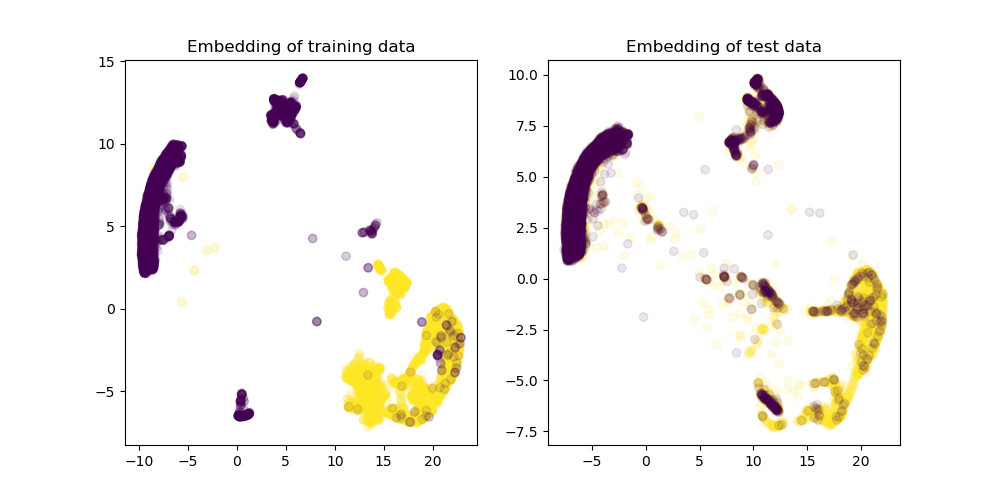
\includegraphics[width=\linewidth]{code_jonas/figures/UMAP_preliminary_classification.png}
    \caption{UMAP classification for the fourier transformed data. 5000 was used to train and 5000 was used to test.}
    \label{fig:UMAP_Classification}
\end{figure}

\textbf{XGB Classifer:}
XGB is an "extreme" gradient boosted decision tree algorithm, ie. an ensemble of decision trees which have been added in a succesive manor in order to complement eachothers weaknesses.
With a straight-out-of-the-box XGB classifier an accuracy of 80\% was achieved for the fourier transformed data.


\subsection{Johann}
I started up making a few out of the box - baseline models. Right now, I'm comparing just the AUC scores for the classification. For baseline we use a max value within the "peak-interval" this gives around AUC $= 0.87$ the XGBoost can out of the  box get performance upwards of $0.88$. I'm just starting to work with Feed forward and LSTM networks but prelimenary results give me an AUC of around $0.91$ which suggests that it is a good way to go. 



\end{document}
